Exact algorithms for the TSP are methods that guarantee finding the optimal solution to the problem by exploring all possible combinations of city tours. These algorithms are based on exhaustive search and systematic enumeration, ensuring that no potential solution is overlooked. While they may work well for small instances of the TSP, they become computationally infeasible for larger problem since it leads to a time complexity of $O(n!)$.


\section{Benders}
Benders' Decomposition is a powerful optimization technique used to solve large-scale combinatorial problems like the Travelling Salesman Problem (TSP). It was introduced by Jacques F. Benders in the 1960s \cite{benders1962} and has since become a widely used approach in the field of mathematical programming.

The Travelling Salesman Problem is known to be a challenging NP-hard problem, meaning that finding the optimal solution for large instances can be computationally intractable using traditional methods like brute-force or exact algorithms. Benders' Decomposition addresses this issue by breaking down the problem into smaller, more manageable subproblems and solving them iteratively.

The basic idea behind Benders' Decomposition is to partition the original problem into a master problem and multiple subproblems. The master problem is an integer linear programming (ILP) relaxation of the original TSP, allowing for the relaxation of some constraints. It aims to find a lower bound on the optimal solution value of the TSP. The subproblems, also known as \textit{Benders' cuts} or \textit{feasibility cuts}, are used to correct the solution obtained from the master problem by adding additional constraints that remove infeasible solutions, called \textit{Subtour Elimination Constraint} (SEC).

\begin{equation*}
    \sum_{e \in E(S_k)} x_e \leq |S_k|-1 \quad \quad \forall S_k: k=1,2,...
\end{equation*}

In the implementation of Algorithm \ref{algo:benders} we use CPLEX to build an initial ILP model of the TSP instance with only the degree equals 2 constraints for each node. We solve this model iteratively to obtain a solution,  which may not be feasible for the original TSP, in the sense that it contains subtours (internal cycles). Each subtour is considered a connected component and we generate Benders' cuts based on these components to eliminate them from consideration in subsequent iterations of the algorithm. We add these cuts to the CPLEX model, called \textit{Subtour Elimination Constraint} (SEC), which tightens the relaxation and improves the solution quality.



\begin{algorithm}
    \caption{Benders Algorithm}\label{algo:benders}
    \begin{algorithmic}[1]
    \Require $G = (V,E), c:E \to \mathbb{R}^+$
    \Ensure $\text{Optimal TSP solution}$
    
    \State $*$ initialize a basic CPLEX model with degree constraints $*$

    \State $ ncomp \gets 0$

    \While{$ !time_{expired} $}

        \State $*$ Solve CPLEX model$*$
        \State $ncomp \gets $ number of connected components

        \If{$ncomp = 1$}
            \State $*$ we found the optimal solution $*$
            \State \Return Solution
        \EndIf

        \State $*$ computes Patching Heuristic $*$

        \ForEach{connected component}

        \State $*$ add SEC $*$

        \EndFor

       

    \EndWhile

    \State \Return best Solution found


    \end{algorithmic}
\end{algorithm}

\subsection{Patching Heuristic}
In the Algorithm \ref{algo:benders} at line 10, we compute the Patching Heuristic.
It is an extension of Benders' Decomposition that aims to improve the quality of solutions obtained by the original Benders' algorithm before it terminates. 

It addresses a limitation of Benders' Decomposition, which may produce solutions with a relatively large optimality gap due to the relaxation of the TSP constraints in the master problem. The patching heuristic helps close this gap by iteratively improving the solution through additional modifications.

At each iteration of Benders, a solution is obtained, but it might still contain subtours due to the relaxation of constraints. The Patching Heuristic aims to identify and remove these subtours from the solution, thus achieving a feasible solution with tighter bound on the optimal solution value.

In our implementation, the Patching Heuristic repairs the current solution with subtours one component at a time until all components are connected. 
Starting from a first component, it tries to find the edge with lowest $\Delta$ (as defined in Equation \ref{eq:delta}) that connect it to a different component, and then merges the two. This process is repeated until all components are merged into a single one.

\begin{figure}[!h]
    \centering
    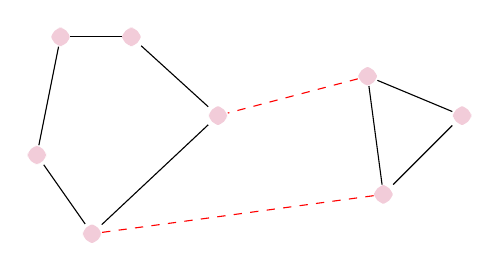
\begin{tikzpicture}
        \tikzstyle{city} = [fill=purple!20,rounded corners]


        \node[city] (A) at (2.3,5.0){};
        \node[city] (B) at (2.6,6.5){};
        \node[city] (C) at (7.7,5.5){};
        \node[city] (D) at (6.7,4.5){};
        \node[city] (E) at (3.0,4.0){};
        \node[city] (F) at (3.5,6.5){};
        \node[city] (G) at (4.6,5.5){};
        \node[city] (H) at (6.5,6){};


        %\draw[->] (C.west) -- (E.east);
        %\draw[->] (B.south) -- (A.east);
        \draw[] (C) edge (D) (E) edge (A) (A) edge (B) (B) edge (F) (F) edge (G) (G) edge (E) (D) edge (H) (H) edge (C);

        \draw[dashed, red] (D) edge (E) (H) edge (G);

    \end{tikzpicture}
    \caption{Example of Patching Heuristic} \label{fig:patch}
\end{figure}




\section{B\&C: Callback For SECs}

A TSP problem can also be solved by the Branch and Cut technique with the help of CPLEX callback functions. Branch and Cut combines the concepts of branch and bound with cutting planes to efficiently explore the solution space and find optimal solutions. The Branch and Cut method begins by solving a relaxation of the original problem. This relaxation (known as LP relaxation) allows fractional solutions, which are not feasible for the original problem, but it provides an upper bound on the optimal solution value.
Next, the algorithm branches on the fractional variables in the LP relaxation, creating multiple subproblems, and then solves each subproblem separately.\\
To speed up the search the method uses valid inequalities (cutting planes) that can be added to the LP relaxation to eliminate fractional solutions, with the result of improving the lower bound on the optimal solution. \\
The Branch and Cut iteratively performs branching, solving LP relaxations, and adding cutting planes until it either finds an optimal solution or proves that no better solution can be found. \\
The CPLEX software can invoke a custom callback (Algorithm \ref{algo:SECcallback}) function whenever a new integer solution is found during the process of searching for a new solution .This solution takes the name of the candidate solution.\\
In this case we check if the solution provided by CPLEX is feasible. Now we are checking if it contains subtours. If the answer is positive, we add SECs for the connected component. \\
The main difference between this approach and Bender’s method is that in this case only a single decision tree is generated.

\begin{algorithm}
    \caption{Callback For SECs}\label{algo:SECcallback}
    \begin{algorithmic}[1]
    \Require TSP solution with subtours
    \State $*$ find subtours that belong to the solution $*$
    \ForEach {subtour  $s \in$ solution}
    \State $*$ add SEC that remove subtour $s *$
    \EndFor
    
    \end{algorithmic}
\end{algorithm}


\section{User Cuts Callback}
This time we present another possible implementation of a CPLEX callback. Now the callback is used in the relaxed solution of the problem. This special type of solution doesn’t consider the integer constraints of the decision variables. \\
The task that this specific callback has to solve is the same as the one presented in the previous section, but the function  is applied on the continuous relaxation of the problem.\\
In order to implement this type of procedure we need the use of the Concorde library, because the solution found is not integer.

We use the function \textit{CCcut\_connect\_components} to find the number of connected components in a fractional solution. Now if there is only one component, it may not be a TSP solution, because it could be still fractional. In this case we use the function \textit{CCcut\_violated\_cuts} in order to cut this solution.\\


\subsection{Tuning of User Cuts Callback}
We cannot apply this type of callback at every node of the branching tree, because it would take too much time to find the solution, due to the high time taken by the algorithms present in the concorde library. So we apply this procedure only if the “number” that identify every node of the branching tree has a particular feature.
Thus the parameter to tune is strictly connected to how many nodes of the branching tree can have the callback applied to.
In Figure \ref{fig:concorde} the numbers tested refer to the ratio of nodes to which the callback is applied. A value of 2 refers to half the nodes, while a value of 10 refers to a tenth of the nodes and so on.

\begin{figure}[!h]
    \centering
    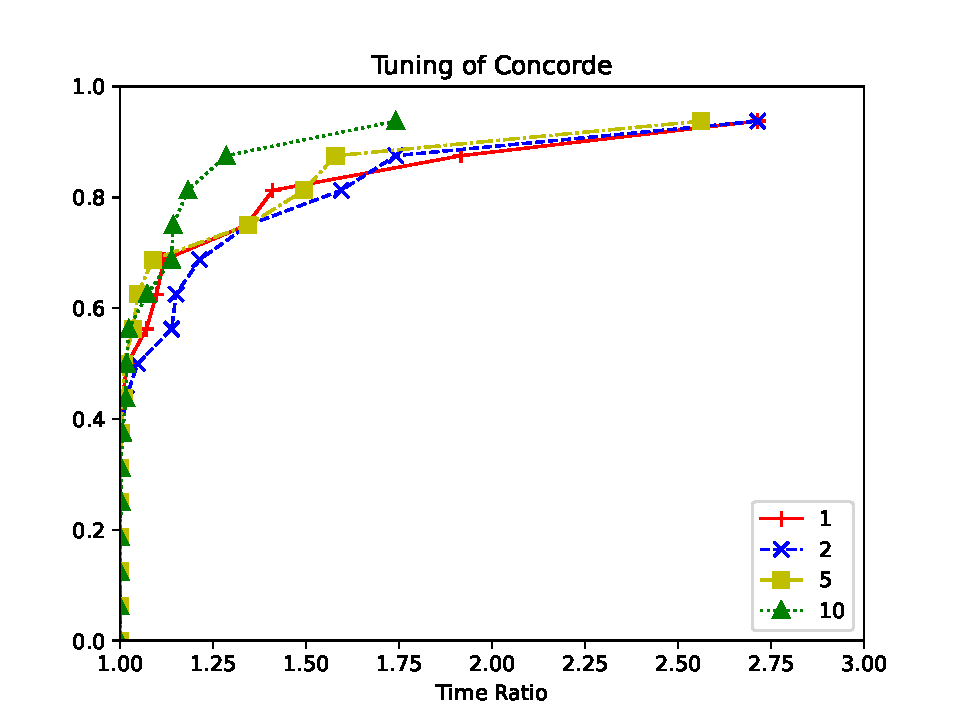
\includegraphics[width=\textwidth]{images/concorde.pdf}
    \caption{Tuning of node ratio in User Cuts Callback}
    \label{fig:concorde}
\end{figure}

\section{Comparison of Exact Methods}

We tested the performance of all three exact methods mentioned above, running on the same instances for 5 minutes each. In Figure \ref{fig:exact} it can be seen that all of them performs really well in 30\% of instances, but the User Cuts Callback using the Concorde library actually outperforms the other methods overall, even if it employs time-consuming routines based on Concorde documentation.

It is quite straightforward why Benders Algorithm performs the worst, since it reconstruct the model at each iteration, wasting more time compared to the other methods.

\begin{figure}[!h]
    \centering
    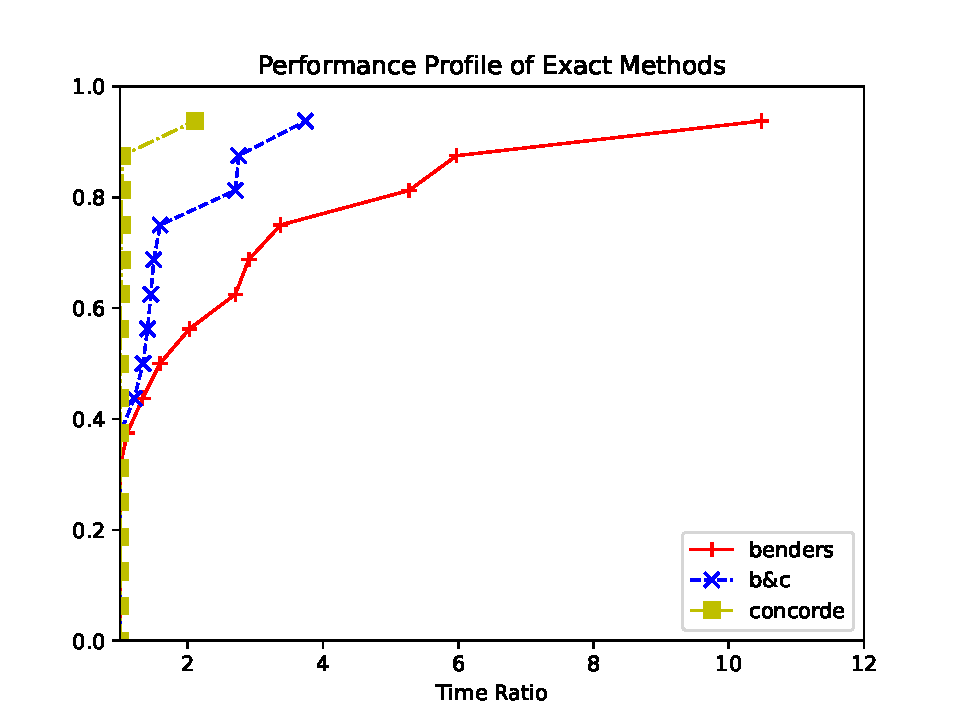
\includegraphics[width=\textwidth]{images/exact.pdf}
    \caption{Performance Profile of Exact Methods}
    \label{fig:exact}
\end{figure}